\RequirePackage[T1]{fontenc}
\documentclass[conference,a4paper]{IEEEtran}
\usepackage{amsmath}
\usepackage{booktabs}
\usepackage{balance}
\usepackage{tikz}
\usepackage{cite}
\usepackage[hidelinks]{hyperref}
\usetikzlibrary{arrows.meta}
\hypersetup{
  pdftitle={Design and implementation of an encrypted instruction set processor on FPGA},
  pdfauthor={George David Tsitlauri},
  pdfsubject={CryptoCPU, BSc thesis, 2025},
  pdfkeywords={encrypted instructions, AES, XEX, processor, FPGA, HLS}
}

\begin{document}

\title{Design and implementation of an encrypted instruction set processor on FPGA}
\author{\IEEEauthorblockN{George David Tsitlauri}
\IEEEauthorblockA{Department of Informatics and Telecommunications\\
University of Thessaly, Greece\\
BSc thesis, 2025}}
\maketitle

\begin{abstract}
CryptoCPU executes AES-128-encrypted programs with a six-stage, in-order
MIPS32-subset processor. Address-dependent AES-XEX protects instruction blocks;
an internal cache reuses decrypted instructions without writing them to memory.
Code, tweak and data-operation keys are separate inputs. The C++ implementation
passes AES known-answer checks, while fourteen directed programs and 5,000
randomized runs agree with a reference interpreter. Three injected pipeline
faults are detected. At the eight-line cache design point, encryption increases
summed modeled cycles across ten benchmarks by 1.5\%, although individual
overhead reaches 133.8\% for a short program. Ciphertext experiments characterize
execution failures without asserting authentication. The thesis prototype was
implemented with Vitis HLS and Vivado on an Artix-7 FPGA and executed an
encrypted program on the board; resource estimates are given for this
configuration.
\end{abstract}

\begin{IEEEkeywords}
encrypted instructions, AES-128, XEX, processor pipeline, FPGA, high-level synthesis
\end{IEEEkeywords}

\section{Introduction}
CryptoCPU studies encrypted execution with a decryption stage between fetch
and decode. Its central idea, originating in the 2025 BSc thesis~\cite{thesis},
is to retain ciphertext in instruction storage, decrypt blocks inside the core,
and cache recovered instructions so that loops amortize the cryptographic work.
The six-stage pipeline, separate memories and assembly/encryption toolchain
preserve this approach. Standard subset encodings, separate keys and reference
state comparison keep the implementation precise and verifiable.

AES supplies the block cipher~\cite{aes}. ECB preserves equality between
repeated plaintext blocks~\cite{modes}, including instruction padding.
Tweakable encryption provides context-dependent transforms~\cite{xex};
CryptoCPU uses XEX with an AES-derived tweak for each nonce and block address.
The contribution is the executable architecture and reproducible evaluation
of its behavior and modeled cost, not a new cipher or authentication scheme.
The repository preserves source, tests, verification manifests and the
original thesis documents.

\section{Architecture and Protection Boundary}
\subsection{Pipeline and Memory Organization}
The stages are instruction fetch (IF), decrypt/cache access (DC), instruction
decode (ID), execute (EX), memory access (MEM) and write-back (WB).
Fig.~\ref{fig:architecture} shows their relationship. Forwarding resolves
supported data dependencies, a load-use detector inserts a stall, and branches
resolve in EX with younger instructions squashed. The ISA uses no branch delay
slots. Faults stop execution at retirement after older instructions complete;
the output state includes the termination status and end PC.

\begin{figure}[t]
\centering
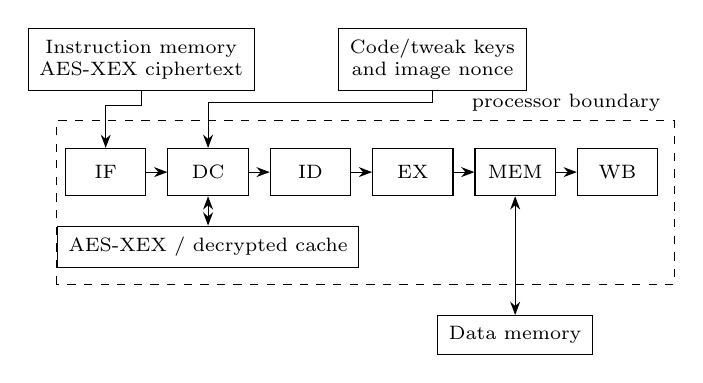
\begin{tikzpicture}[x=1cm,y=1cm,font=\scriptsize,>=Stealth,
  stage/.style={draw,minimum width=1.02cm,minimum height=0.60cm,align=center},
  box/.style={draw,align=center,inner sep=4pt}]
  \draw[dashed] (-0.03,-0.78) rectangle (7.82,1.30);
  \node[anchor=south east] at (7.77,1.30) {processor boundary};
  \node[stage] (if) at (0.60,0.65) {IF};
  \node[stage] (dc) at (1.90,0.65) {DC};
  \node[stage] (id) at (3.20,0.65) {ID};
  \node[stage] (ex) at (4.50,0.65) {EX};
  \node[stage] (mem) at (5.80,0.65) {MEM};
  \node[stage] (wb) at (7.10,0.65) {WB};
  \foreach \a/\b in {if/dc,dc/id,id/ex,ex/mem,mem/wb}
    \draw[->] (\a) -- (\b);
  \node[box] (imem) at (1.05,2.08) {Instruction memory\\AES-XEX ciphertext};
  \node[box] (keys) at (4.75,2.08) {Code/tweak keys\\and image nonce};
  \draw[->] (imem.south) -- (1.05,1.50) -| (if.north);
  \draw[->] (keys.south) -- (4.75,1.53) -| (dc.north);
  \node[box] (cache) at (1.90,-0.30) {AES-XEX / decrypted cache};
  \draw[<->] (dc.south) -- (cache.north);
  \node[box] (dmem) at (5.80,-1.42) {Data memory};
  \draw[<->] (mem.south) -- (dmem.north);
\end{tikzpicture}
\caption{Logical instruction path. Plaintext instruction blocks remain inside
the core. AES data instructions operate through MEM using a separate data key.}
\label{fig:architecture}
\end{figure}

The supported MIPS32 subset includes arithmetic, logic, shifts, multiply/divide
with HI/LO, byte/halfword/word loads and stores, branches, jumps and calls.
Instruction storage contains 4,096 words at base address \texttt{0x00400000};
data storage contains 4,096 words at \texttt{0x10010000}. Each is 16~KiB.
The stack starts at the end of data memory. These addresses follow the MARS
convention, without implying complete MIPS compatibility.

Four instructions form a 128-bit AES block. The direct-mapped decrypted cache
has eight active lines by default: 128 bytes of instruction data, excluding
tags. Supported configurations use powers of two from one to 64 lines.
The C++ arrays reserve the maximum capacity, so an active-line setting alone
does not determine synthesized storage. The core exposes instruction memory
as a read-only input and has no write path that copies decrypted instructions
into data memory. Plaintext appears in its cache, pipeline and internal
temporaries.

\subsection{Instruction Encryption and Separate Keys}
Let $P_b$ and $C_b$ denote plaintext and ciphertext at block index $b$.
The repository image format uses
\begin{align}
  T_b &= E_{K_t}(N_0\,\|\,N_1\,\|\,0\,\|\,b), \\
  C_b &= E_{K_c}(P_b \oplus T_b) \oplus T_b, \\
  P_b &= D_{K_c}(C_b \oplus T_b) \oplus T_b.
\end{align}
Here $E$ and $D$ are AES-128 encryption and decryption, $K_c$ is the code key,
and $K_t$ is the tweak key. Each concatenated field is 32 bits; $N_0,N_1$
form a public 64-bit image nonce. Words enter AES in most-significant-byte-first
order. This is a defined AES-XEX block format, not an XTS storage format.
Encryption remains deterministic at a fixed key, nonce and block index;
different images should use distinct nonces when the key pair is reused.

A third key, $K_d$, serves the private \texttt{aesenc} and \texttt{aesdec}
instructions (opcodes \texttt{0x3A} and \texttt{0x3B}). They transform a 16-byte
block in data memory, using source and destination addresses held in registers.
Separate data and code keys prevent this interface from directly decrypting
instruction ciphertext. Ordinary data memory is otherwise unencrypted.

\subsection{Threat Model}
The adversary may inspect or modify instruction ciphertext, but cannot access
internal plaintext or code/tweak keys. Hardware provisioning, access control
and debug restrictions enforce that boundary; a C++ key argument alone cannot.
XEX has no authentication tag, and corrupted plaintext may decode into valid
instructions. Traps therefore do not establish integrity. Replay, access
patterns, compromised provisioning and physical side channels are outside the
evaluated protection.

\section{Implementation and Evaluation Method}
\subsection{Software and Reference Execution}
The C++17 design uses fixed-size arrays and HLS top function
\texttt{cryptocpu\_top}. The toolchain includes an assembler, image tool,
sequential reference interpreter and self-checking testbenches. The interpreter
independently implements decode/execute but shares the AES routines;
known-answer tests provide the separate cryptographic check. Data-label
alignment and strict key-file/argument handling have targeted regressions.

The directed testbench compares status, end PC, retired count, all 32 general
registers, HI/LO and complete data memory; fixed expected values additionally
check intended program behavior. Source/binary hashes, commands, versions,
exit codes and actual verification timestamps are recorded in
\texttt{results/host/manifest.json}. The recorded run uses Python~3.13.16
and LLVM-MinGW/Clang~23.1.1 on Windows.

\subsection{Cycle Accounting}
One main-loop iteration is one modeled pipeline cycle. At the design point,
an instruction-block miss costs a four-cycle memory delay plus an eleven-cycle
AES service delay when encryption is enabled. A cache hit reuses the decrypted
block without this service. The plaintext baseline retains the same pipeline,
cache and memory delay. Data AES instructions use the configured AES latency.

These parameters abstract implementation timing. In particular, the model does
not separately schedule tweak derivation and block decryption; setup and key
expansion precede cycle accounting, and multiply/divide execute in one modeled
cycle. An HLS schedule need not map a model iteration to one FPGA clock cycle.
Performance is reported as cycles and cycles per retired instruction (CPI),
without converting it into a physical frequency or throughput.

\subsection{Test Campaigns}
AES encryption and decryption are checked against FIPS-197 examples and four
SP~800-38A AES-128 blocks~\cite{aes,modes}; 10,000 randomized XEX round trips
check inversion. Fourteen directed programs exercise computation, dependencies,
control flow, AES operations, data alignment and three exception cases.
Random differential testing generates 1,000 programs using seed 2026 and runs
each in five configurations. Mutation testing deliberately removes forwarding,
a load-use stall or a branch squash, with 100 programs in five configurations
per mutant (seed 7).

For ciphertext experiments, ten programs are executed with a wrong code key,
500 single-bit flips each (seed 1), and pairs of swapped code blocks.
Classification distinguishes traps, timeouts, normally halted changed states
and normally halted unchanged states. Comparison includes PC and HI/LO as well
as registers and memory. The timeout budget is $20C+1000$ modeled cycles for
baseline cost $C$. The bit-flip sequence uses the C runtime's \texttt{rand()},
so exact samples depend on the recorded runtime as well as the seed.

\section{Results and Discussion}\label{sec:results}
\subsection{Functional Checks}
Table~\ref{tab:verification} summarizes the host results. All directed programs
pass. Random execution produces 4,455 normal halts, 430 memory traps and 115
overflow traps, with zero mismatches against the reference. The targeted
tooling tests include multiple invalid-input subcases; the outcome-classifier
tests include programs differing only in HI, LO or end PC.

\begin{table}[t]
\caption{Host verification results}
\label{tab:verification}
\centering
\small
\begin{tabular}{@{}ll@{}}
\toprule
Check & Observed result \\
\midrule
AES known-answer vectors & All pass, both directions \\
XEX randomized round trips & 10,000 pass \\
Directed programs & 14/14 pass \\
Random differential runs & 5,000; zero mismatches \\
Tooling / classification regressions & 6 methods / 8 cases pass \\
Forwarding mutant & Detected in 500/500 runs \\
Load-use mutant & Detected in 405/500 runs \\
Branch-squash mutant & Detected in 495/500 runs \\
\bottomrule
\end{tabular}
\end{table}

The three detected mutants establish sensitivity to those defects, not
exhaustive correctness.

\subsection{Ciphertext Observations}
Across the ten benchmark images, XEX produces 1,024 distinct ciphertext blocks
per 16-KiB image. ECB preserves the 4--11 distinct plaintext patterns present
in each image, including padding. The directed-test memory scan finds no
complete, nonzero 16-byte instruction blocks in the ciphertext image or final
data memory. This check does not address fragments, transient leakage or
physical observation.

\begin{table}[t]
\caption{Observed ciphertext-modification outcomes}
\label{tab:tamper}
\centering
\small
\begin{tabular}{@{}lrrrr@{}}
\toprule
Experiment & Runs & Traps & Timeouts & Changed halt \\
\midrule
Wrong code key & 10 & 10 & 0 & 0 \\
Single-bit flip & 5,000 & 4,995 & 5 & 0 \\
Block swap & 208 & 208 & 0 & 0 \\
\bottomrule
\end{tabular}
\end{table}

Table~\ref{tab:tamper} records 99.9\% traps and 0.1\% timeouts for bit flips;
no modified run halts with a changed or unchanged final state. These sampled
outcomes do not establish arbitrary-tamper detection for an unauthenticated
format.

\balance
\subsection{Modeled Performance}
Table~\ref{tab:performance} compares the same workloads with and without
instruction encryption. All use a cold cache, eight active lines, four-cycle
memory reads and eleven-cycle AES service. The encrypted total is 46,773
cycles versus 46,068 plaintext cycles: an increase of 705 cycles, or 1.5\%.
This ratio is computed from summed cycles, not from an unweighted mean of
per-program overheads; Fibonacci dominates the aggregate execution time.

\begin{table}[t]
\caption{Cycle-model performance at the design point}
\label{tab:performance}
\centering
\small
\begin{tabular}{@{}lrrrr@{}}
\toprule
Program & Retired & Plain cycles & XEX cycles & Increase \\
\midrule
Signature & 16 & 37 & 81 & 118.9\% \\
Loop sum & 408 & 722 & 755 & 4.6\% \\
Fibonacci & 19,731 & 36,532 & 36,609 & 0.2\% \\
Bubble sort & 957 & 1,562 & 1,628 & 4.2\% \\
Strings & 171 & 311 & 377 & 21.2\% \\
Mul/div & 33 & 74 & 173 & 133.8\% \\
AES data & 11 & 45 & 68 & 51.1\% \\
Hazards & 37 & 91 & 179 & 96.7\% \\
Sieve & 3,174 & 5,250 & 5,349 & 1.9\% \\
Matrix multiply & 1,146 & 1,444 & 1,554 & 7.6\% \\
\midrule
Total & 25,684 & 46,068 & 46,773 & 1.5\% \\
\bottomrule
\end{tabular}
\end{table}

The five loop-oriented benchmarks incur 0.2--7.6\% overhead. Short programs
pay proportionally more for initial misses: the 33-instruction multiply/divide
benchmark rises from 74 to 173 cycles. The cache-size sweep exposes the same
tradeoff. With one active line, the loop-oriented workloads have CPI values
of 5.911--9.130; with eight lines, they reach 1.356--1.855. Increasing capacity
past eight lines does not improve these small benchmark results.

The latency sweep varies modeled AES service from one to 44 cycles. Fibonacci
changes only from 1.853 to 1.867 CPI at eight lines, whereas the short
multiply/divide program changes from 2.515 to 14.242 CPI. Consequently, the
measured model advantage comes from locality and reuse; it does not predict
the overhead of arbitrary applications or a specific AES hardware design.

\section{FPGA Implementation}
\subsection{Thesis Prototype}
The thesis prototype~\cite{thesis} followed the complete Vitis HLS and Vivado
flow~\cite{hls,vivado}. C simulation executed the encrypted demonstration
program and passed its signature check; C synthesis produced the RTL, and
C/RTL co-simulation reproduced the C-simulation signature, register dump and
memory dump. The core was packaged as an IP block and placed in a Vivado
block design with a clocking wizard, a processor-system reset and a constant
\texttt{ap\_start}. Its \texttt{ap\_done} output drives an LED.

The design was implemented on an AMD Artix-7 XC7A200T (AC701 evaluation
board), with the 200~MHz differential system clock on pins R3/P3 and the LED
on pin M26. Timing closed with positive slack, and the bitstream ran the
encrypted program on the board, where the LED confirmed completion.
Table~\ref{tab:fpga} lists the implementation results. That prototype
decrypted instruction blocks with AES-128 in ECB mode.

\begin{table}[b]
\caption{Artix-7 XC7A200T implementation}
\label{tab:fpga}
\centering
\small
\begin{tabular}{@{}lrr@{}}
\toprule
Quantity & Thesis prototype & This configuration \\
 & (measured) & (estimated) \\
\midrule
Clock & 75~MHz & 75~MHz \\
LUTs & ${\approx}15\%$ & 15--17\% \\
Flip-flops & ${\approx}10\%$ & 10--11\% \\
Block RAM & ${\approx}12\%$ & ${\le}12\%$ \\
DSP slices & ${\approx}5\%$ & ${\approx}5\%$ \\
Power (Vivado estimate) & ${\approx}0.6$~W & ${\approx}0.6$~W \\
\bottomrule
\end{tabular}
\end{table}

\subsection{Estimated Cost of This Configuration}
The estimates in Table~\ref{tab:fpga} start from the prototype and account for
the differences in the datapath. The pipeline, register file, forwarding and
memory interfaces are unchanged. XEX adds one AES encryption per instruction
block to derive the tweak, together with a 128-bit tweak register and two
128-bit XOR stages; when the tweak reuses the iterative AES round logic, the
added area is mainly registers and multiplexing, about 1--2\% of the device's
LUTs. The decrypted cache of eight 16-byte lines is smaller than the
prototype's 4~KiB instruction cache, so block-RAM use does not grow. The
critical path remains in the AES round and the execute stage, so the clock
estimate follows the prototype. These figures are estimates, not reports of
an implementation of this configuration.

\section{Conclusion}
CryptoCPU preserves the original encrypted-execution idea through separate
keys, address-dependent encryption, standard subset decoding and stronger
verification. The evaluated programs agree with the reference, while a small
decrypted cache amortizes modeled AES cost through reuse. Authentication and
physical protection remain distinct concerns.

Crypto3DStackCPU~\cite{crypto3d} continues this direction
through a four-tier memory model, encrypted and authenticated program images,
and protected transfers between tiers. It has its own implementation and
validation; CryptoCPU provides the encrypted-instruction foundation.

\bibliographystyle{IEEEtran}
\bibliography{references}
\end{document}
